\section{Methodology}


\subsection{Introduction to UCF101 Dataset}
The \textbf{UCF101} dataset \cite{soomro2012ucf101} serves as a fundamental benchmark for action recognition research in computer vision. It provides a diverse collection of \textbf{13,320 video clips} curated from YouTube, encompassing a wide array of human activities across \textbf{101 distinct action classes} (showned in Figure~\ref{fig:ucf101}). These classes range from fine-grained daily tasks, such as \textit{Brushing Teeth} or \textit{Applying Makeup}, to complex athletic maneuvers and musical performances.\\\\
The 101 categories are taxonomically organized into five primary types based on the nature of the movement and the entities involved:
\begin{itemize}
    \item \textbf{Human-Object Interaction:} Actions involving tools or equipment (e.g., Knitting, Hammering).
    \item \textbf{Body-Motion Only:} Purely physical movements without external objects (e.g., Baby Crawling, Jumping Jacks).
    \item \textbf{Human-Human Interaction:} Actions requiring multiple participants (e.g., Salsa Spin, Fencing).
    \item \textbf{Playing Musical Instruments:} Highly rhythmic and localized movements (e.g., Playing Cello, Playing Flute).
    \item \textbf{Sports:} Dynamic actions performed in specific athletic environments (e.g., Archery, Basketball Dunk).
\end{itemize}
\noindent
A defining structural feature of UCF101 is its hierarchical organization. Within each category, videos are partitioned into \textbf{25 distinct groups}, each containing \textbf{4 to 7 clips}. Videos belonging to the same group typically share significant contextual features, such as similar backgrounds, consistent viewpoints, and common subjects \cite{soomro2012ucf101}.

\begin{figure}[h]
    \centering
    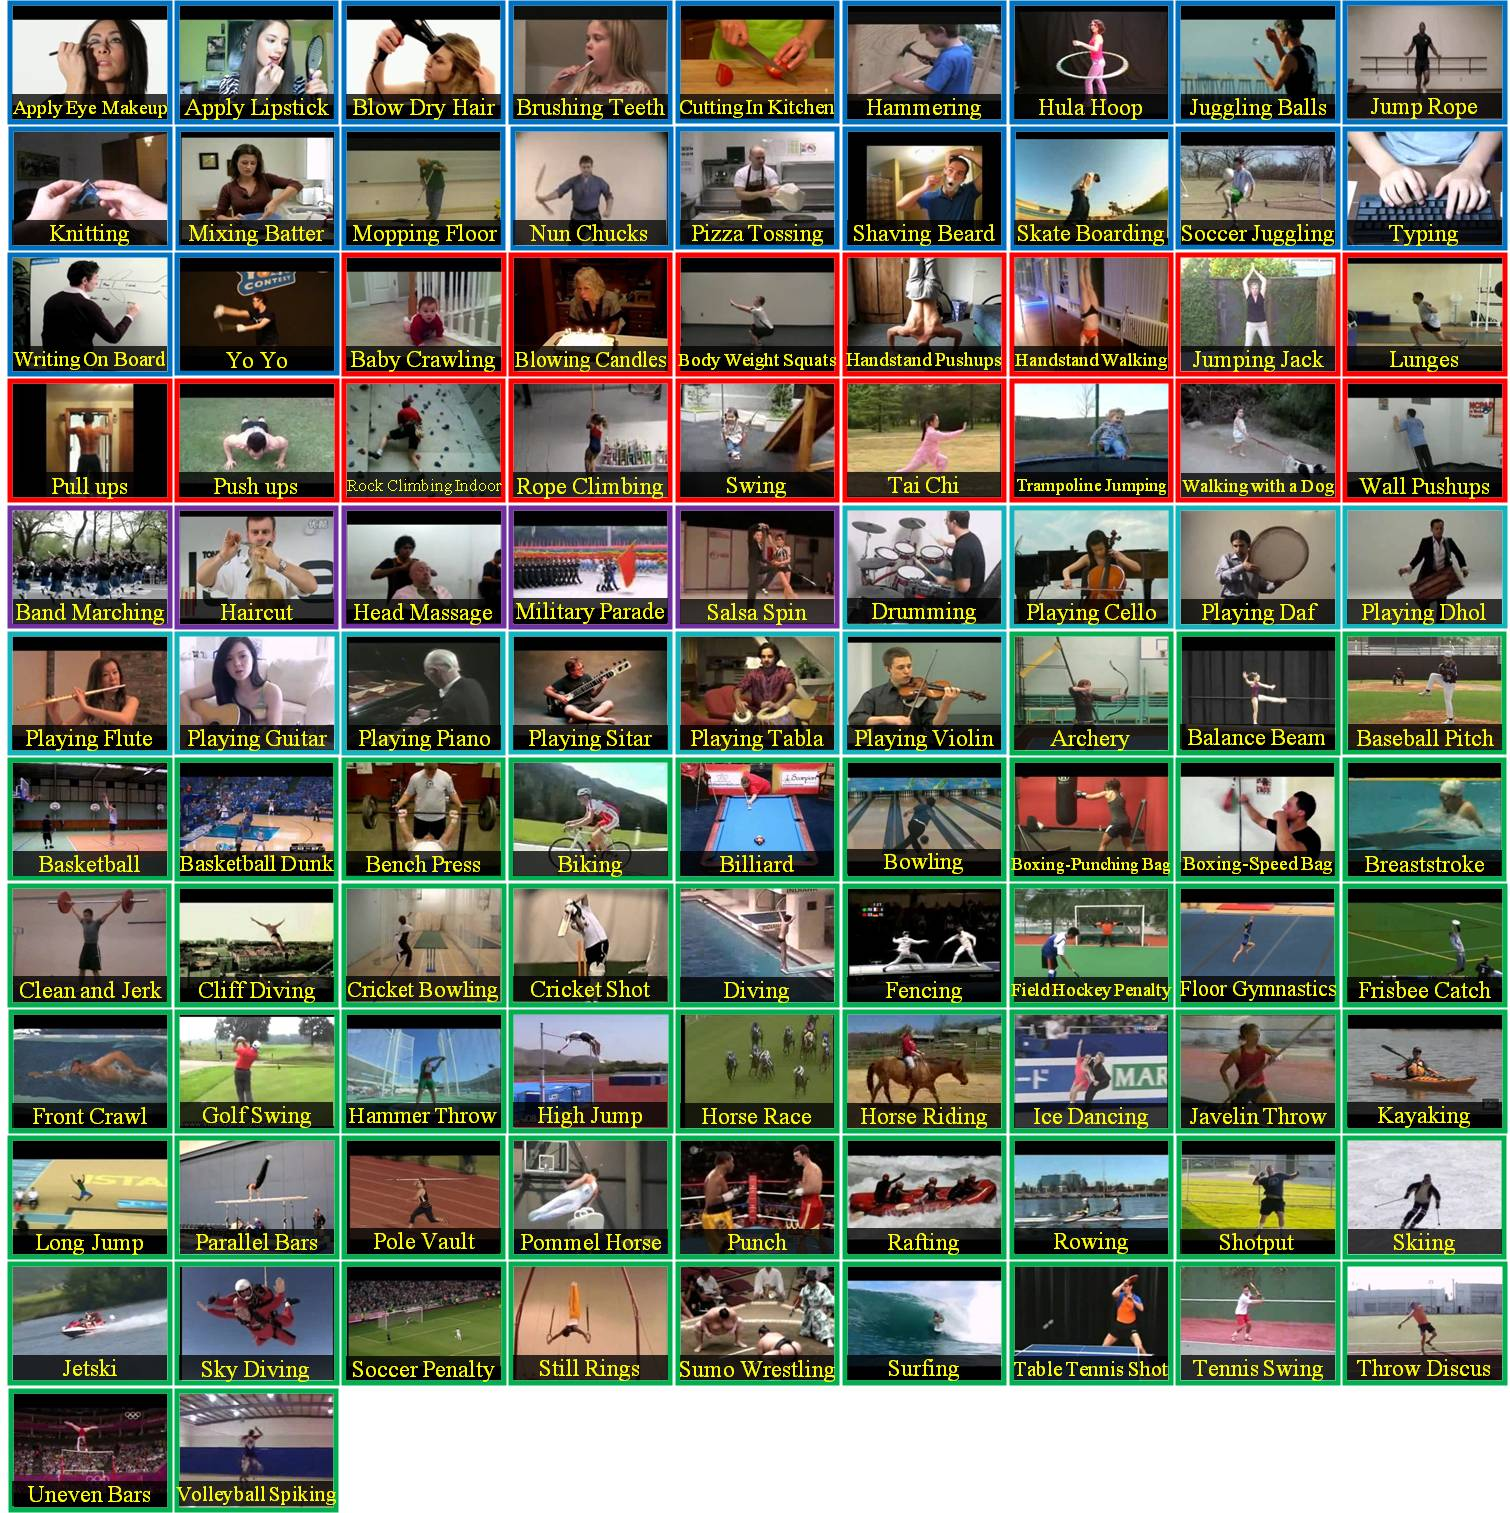
\includegraphics[width=0.5\textwidth]{images/classes.png}
    \caption{A representative frame for each action class in the UCF101 dataset. \cite{ucf101_website}.}
    \label{fig:ucf101}
\end{figure}


\subsection{Class Distribution Analysis}
Figure~\ref{fig:ucf101_cd} presents the distribution of video samples across the 101 action classes of the UCF101 dataset. The bar chart highlights a moderate degree of class imbalance: the most frequent class, \textit{Punch}, contains 121 samples, while the least represented class, \textit{TaiChi}, includes 72 samples. On average, each class is represented by approximately 94.4 video samples. Despite the non-uniform distribution, the ratio between the majority and minority classes remains below 2:1, indicating that the imbalance is relatively mild.\\
From a training perspective, this level of imbalance does not warrant the use of aggressive compensation techniques such as synthetic oversampling (e.g., SMOTE) or class-weighted loss functions. Instead, random shuffling is employed within the \texttt{DataLoader} to ensure that each mini-batch contains a stochastic mixture of action classes. This strategy reduces the risk of the model developing a bias toward more frequent actions during the gradient descent optimization process, while preserving the original data distribution.

\begin{figure}[h]
    \centering
    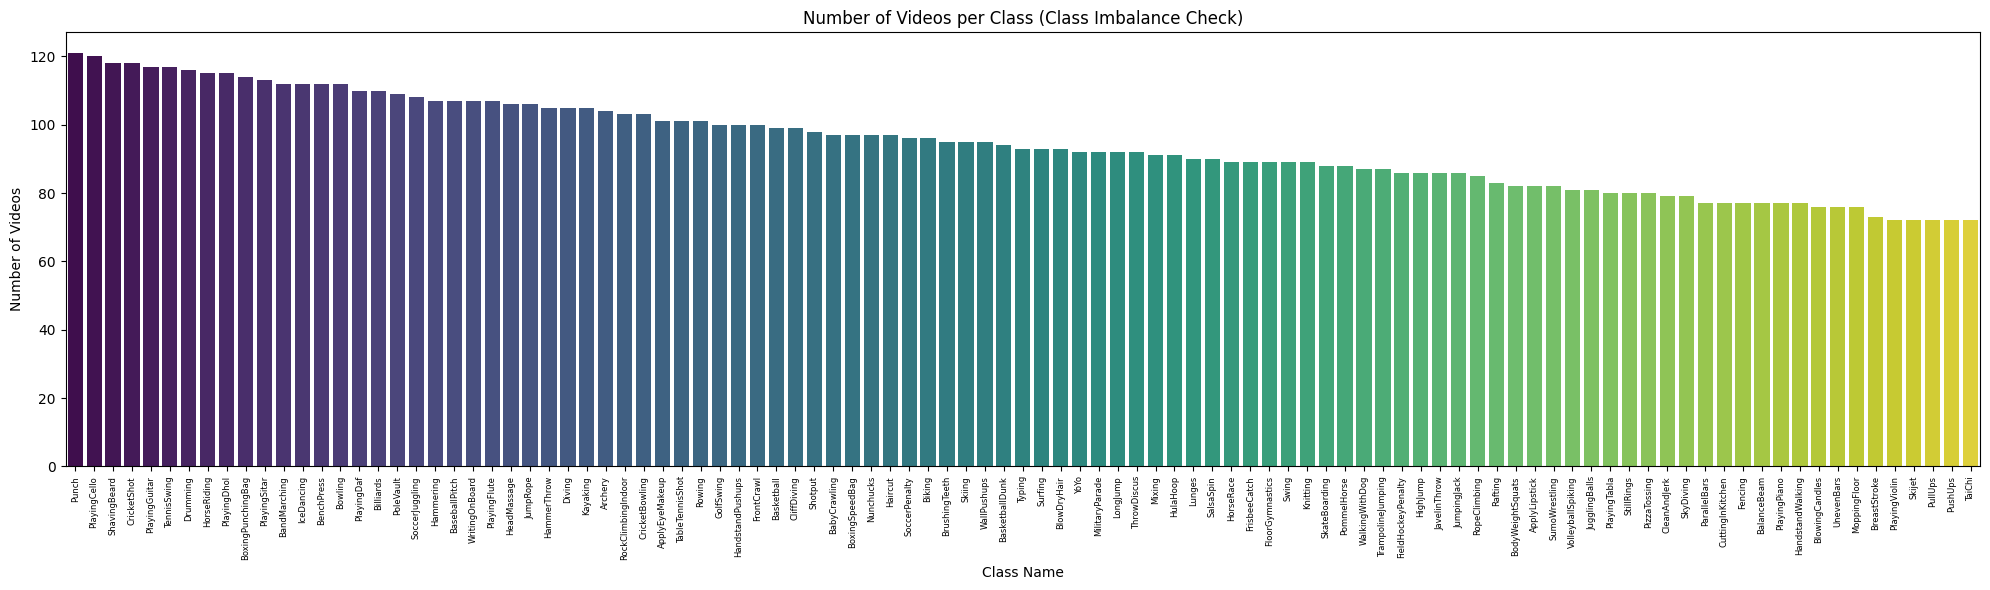
\includegraphics[width=1\textwidth]{images/CD.png}
    \caption{Class Distribution in UCF101 Dataset.}
    \label{fig:ucf101_cd}
\end{figure}

\subsection{Data Splitting and Integrity}
The division of the dataset follows a rigorous protocol to ensure the reliability of the results. While the training and test sets are provided directly by the original UCF101 creators \cite{soomro2012ucf101}, the validation set was extracted from the training partition using a \textbf{group-wise splitting strategy}.
This approach is fundamental to prevent \textbf{data leakage}: since videos in the same group often share the same subject, background, and camera viewpoint, a random split would allow the model to "memorize" specific environments. By isolating groups, the model is forced to generalize to unseen subjects and settings. Finally, an integrity check was performed post-split, confirming zero overlapping samples between the training, validation, and test sets, thus guaranteeing an honest assessment of the model's performance.

\subsection{Data Preprocessing and Pipeline}
To process the video data efficiently while preserving spatio-temporal information, the following preprocessing steps were implemented.

\subsubsection{I/O Optimization}
To mitigate the I/O bottleneck—a common challenge when handling thousands of video files—all extracted frames were converted and stored in \textbf{JPEG format}. This optimization significantly reduced disk read times during the training phase, allowing for a higher throughput of samples per second and ensuring that the GPU remains the primary computational bottleneck rather than the storage subsystem.

\subsubsection{Data Augmentation and Spatial Transformation}
To enhance the model's ability to generalize and to mitigate the spatial memorization often observed in high-capacity architectures, a dual-stage transformation pipeline was implemented:
\begin{itemize}
    \item \textbf{Training Augmentation:} During the training phase, \textbf{Random Horizontal Flips} ($p=0.5$) and \textbf{Color Jittering} (adjusting brightness and contrast by $10\%$) were applied. 
    \item \textbf{Standardized Preprocessing:} All frames across all sets were resized to a spatial resolution of $224 \times 224$ pixels. A standard normalization using mean $\mu = [0.485, 0.456, 0.406]$ and standard deviation $\sigma = [0.229, 0.224, 0.225]$, derived from the ImageNet dataset, was applied to align the input distribution with the pre-trained ResNet18 feature space.
\end{itemize}

\subsubsection{Temporal Sampling}
Video was reduced from its native length to a fixed temporal depth of $T=16$ frames. This represents significant a compression. The reasoning behind this choice is twofold:
\begin{enumerate}
    \item \textbf{High Temporal Redundancy:} Adjacent frames in video data are highly correlated and often contain minimal distinct semantic information. Processing every frame would lead to computational inefficiency and potential overfitting without a proportional gain in feature quality.
    \item \textbf{Global Uniform Sampling:} Rather than simple truncation (taking only the first few seconds), the pipeline employs a uniform sampling function. By extracting frames at equidistant intervals across the \textit{entire duration} of the clip, the model captures the full temporal evolution of the action, including the \textbf{onset, nucleus, and offset} phases.
\end{enumerate}
\noindent
This strategy ensures that the resulting tensor, with dimensions $(Batch \times 3 \times 16 \times 224 \times 224)$, remains compatible with GPU memory constraints while preserving the global context of the video sequence.

\subsection{Models}
Several models were implemented, ranging from a custom baseline to state-of-the-art attention-based architectures.

\subsubsection{Custom CNN with temporal mean pooling}
The initial phase of the study involves the design and implementation of a lightweight, shallow Convolutional Neural Network (CNN). This model serves as the experimental baseline, providing a performance floor against more sophisticated architectures.

\subsubsection*{Architectural Design}

The model in Figure~\ref{fig:cnn_custom} is composed of four sequential convolutional blocks. Each block follows a modular design: a 2D Convolutional layer with a $3 \times 3$ kernel, followed by \texttt{Batch Normalization} (BN) to stabilize training, a \texttt{ReLU} activation function, and a \texttt{MaxPool} layer for spatial downsampling.
The spatial resolution of the input frames evolves as follows:
\[
(3 \times 224 \times 224) \xrightarrow{\text{Block 1}} (32 \times 112 \times 112) \xrightarrow{\text{Block 2}} (64 \times 56 \times 56) \xrightarrow{\text{Block 3}} (128 \times 28 \times 28) \xrightarrow{\text{Block 4}} (256 \times 14 \times 14)
\]
A critical design choice is the inclusion of an \textbf{Global Average Pooling} (GAP) layer before the classification head. Instead of a standard flattening of the $256 \times 14 \times 14$ tensor—which would result in a massive fully connected layer ($50,176$ neurons). The GAP layer collapses the spatial dimensions into a $1 \times 1$ representation.

\begin{figure}[h]
    \centering
    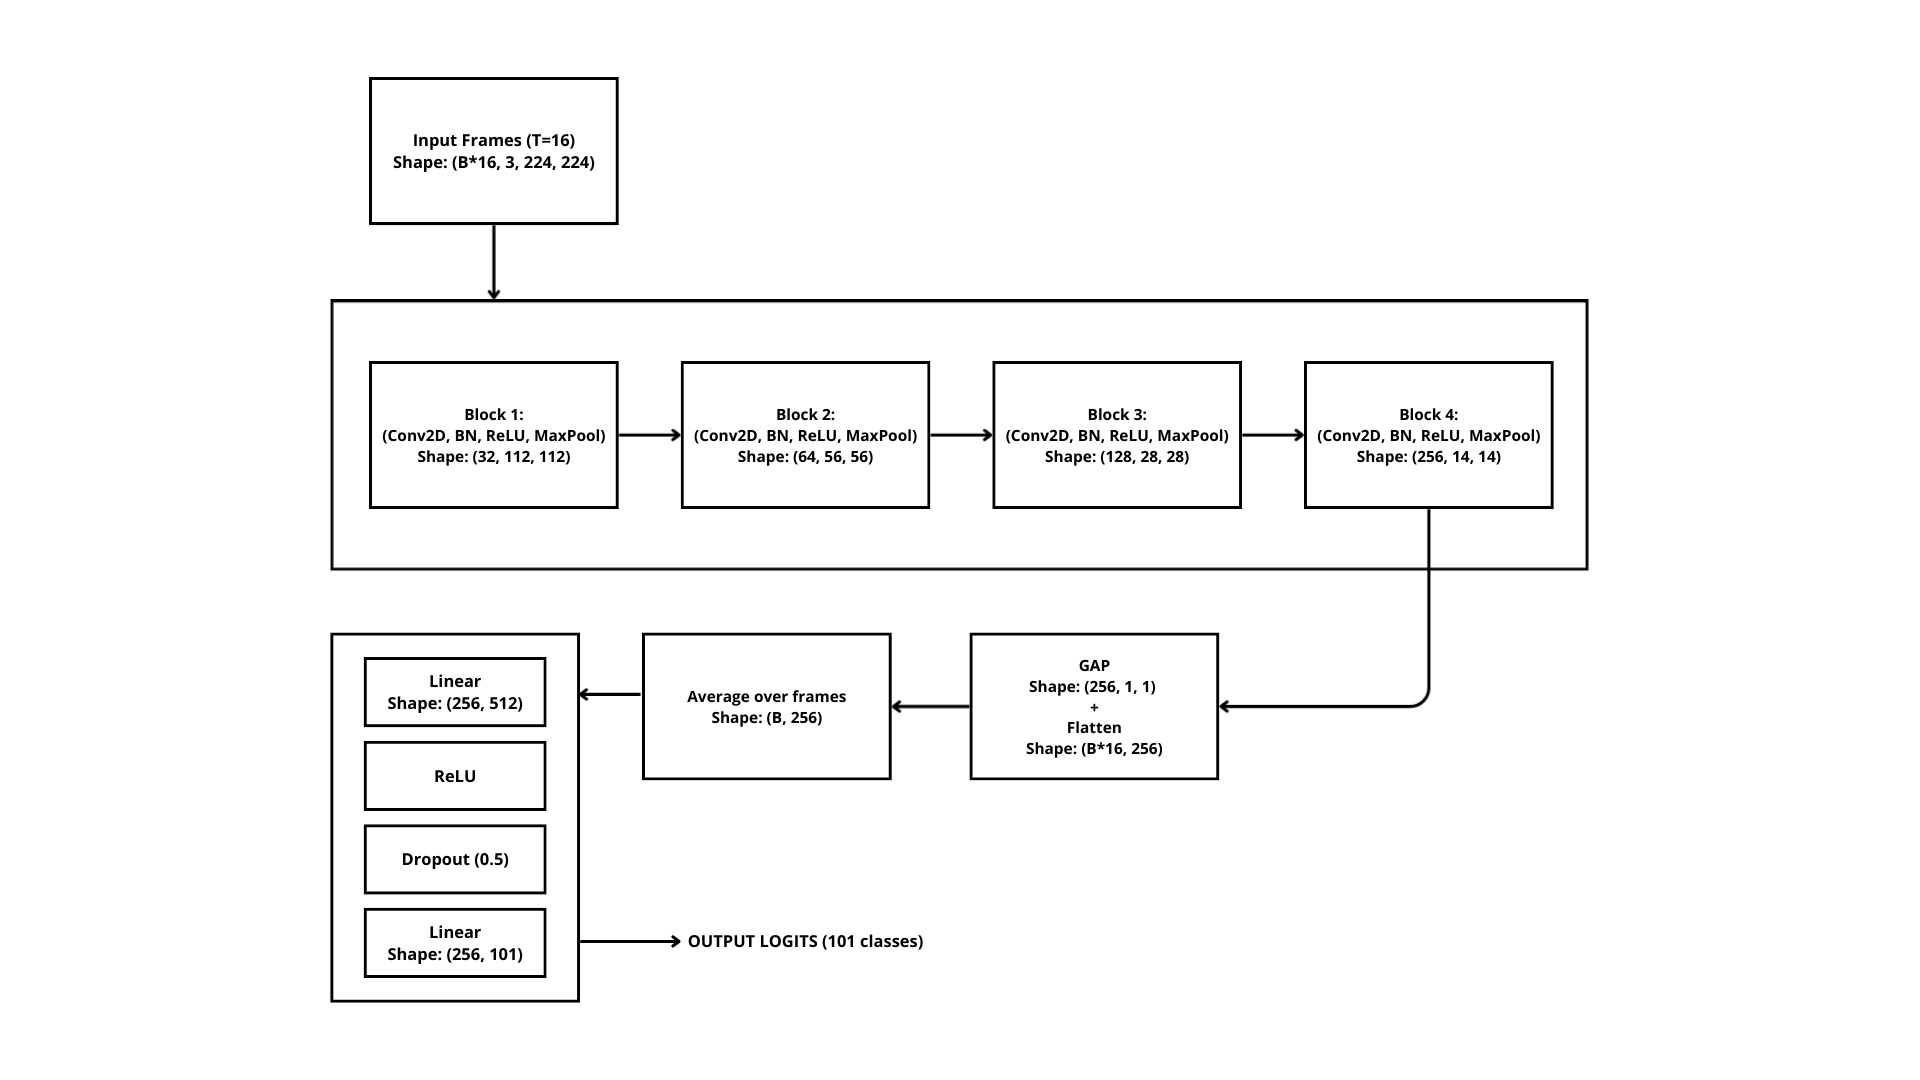
\includegraphics[width=1\textwidth]{images/CNN custom.png}
    \caption{Custom CNN Architecture.}
    \label{fig:cnn_custom}
\end{figure}
\noindent
After the GAP layer the model performs a \textbf{temporal mean pooling} across the sequence:$$ \mathbf{x}_{video} = \frac{1}{T} \sum_{t=1}^{T} \mathbf{x}_t $$
This aggregated vector $\mathbf{x}_{video}$ is then passed to the classification head. This "Bag-of-Frames" approach allows the model to capture the global visual context of the clip, although it remains invariant to the specific chronological order of the actions.


\subsubsection{ResNet18 Backbone with mean temporal pooling}

To overcome the structural limitations and the lack of representational depth of the custom baseline, we transition to a significantly more robust architecture based on ResNet18. This model is architecturally optimized for large-scale image recognition and is far better suited for the high-dimensional complexity of the UCF101 dataset. The primary advantages of this approach include the increased depth of the network, its ability to extract features, and the strategic use of \textbf{Transfer Learning} via weights pre-trained on the ImageNet-1K dataset.

\subsubsection*{Architectural Design}

The architecture of the proposed model, is built upon a modular design that balances feature reuse with specialized \textbf{fine-tuning}.
\begin{enumerate} 
    \item \textbf{Feature Extraction Backbone}: The model adopts a \textbf{ResNet18} architecture as its core feature extractor. 
    \item \textbf{Selective Layer Freezing}: To preserve the general-purpose visual features (such as edges and basic textures) while reducing the number of trainable parameters, a selective freezing strategy is applied. The initial convolutional layer (\texttt{conv1}), the first batch normalization layer (\texttt{bn1}), and the first two residual blocks (\texttt{layer1}, \texttt{layer2}) are frozen. Training is focused exclusively on the deeper layers which are responsible for capturing more abstract and task-specific semantic information.
    \item \textbf{Robust Classification Head}: The original fully connected layer of the ResNet is replaced with a custom module that incorporates a \textbf{Dropout} layer with a probability of $0.5$ that acts as a critical regularizer, followed by a final \textbf{Linear} layer mapping to the 101 classes of UCF101. 
    \item \textbf{Spatiotemporal Processing Pipeline}: The temporal dimension is aggregated via temporal mean pooling, keeping the model invariant to the chronological order of the sequence. 
\end{enumerate}

\subsubsection{ResNet18 + LSTM}
This architecture builds upon the ResNet18 backbone described previously but introduces an LSTM to capture the temporal evolution of the actions by processing the frames as a chronological sequence.

\subsubsection*{Architectural Design}

\begin{enumerate} 
    \item \textbf{Feature Extraction Backbone}: The ResNet18 architecture is employed as a spatial feature extractor, specifically fine-tuned on the UCF101 dataset.
    \item \textbf{Regularization}: a \textbf{Spatial Dropout} is applied immediately after the backbone to regularize the transition to the temporal module and mitigate overfitting.
    \item \textbf{LSTM Module}: A 2-layer \textbf{Unidirectional LSTM} with a hidden size of 1024 is utilized. It processes the sequence of 16 frames to model long-term temporal dependencies.
    \item \textbf{Temporal Aggregation}: The hidden states across the entire sequence are aggregated via \textbf{temporal mean pooling}:
    \[ \mathbf{h}_{pooled} = \frac{1}{T} \sum_{t=1}^{T} \mathbf{h}_t \]
    \noindent
    This ensures the final representation accounts for the whole sequence rather than just the last frame.
    \item \textbf{Classification Head}: A sequential MLP (Linear 1024 $\to$ 512, ReLU, Dropout 0.5, Linear $\to$ 101) for the final class prediction.
\end{enumerate}

\subsubsection{ResNet18 + BiLSTM}

This architecture upgrades the temporal module to a \textbf{Bidirectional LSTM (BiLSTM)}, allowing the network to capture dependencies from both past and future frame contexts simultaneously.

\begin{enumerate} 
    \item \textbf{Feature Extractor}: ResNet18 backbone (ImageNet pre-trained) for frame-level extraction, with full fine-tuning of all parameters enabled.
    \item \textbf{Regularization}: a \textbf{Spatial Dropout} is applied to the feature sequence to prevent overfitting.
    \item \textbf{BiLSTM Module}: a 2-layer Bidirectional LSTM with a hidden size of 512. The bidirectional configuration doubles the output dimensionality to 1024 by concatenating forward and backward hidden states.
    \item \textbf{Temporal Aggregation}: Global average pooling (mean) is performed across the temporal dimension to aggregate the BiLSTM outputs.
    \item \textbf{Classification Head}: A sequential MLP (Linear 1024 $\to$ 512, ReLU, Dropout 0.5, Linear $\to$ 101) for the final prediction.
\end{enumerate}

\subsubsection{Transformer-based Model: VideoMAE}

The VideoMAE (Video Masked Autoencoder) architecture represents a shift toward self-supervised, attention-based spatiotemporal modeling. VideoMAE utilizes a Vision Transformer (ViT) backbone to capture global dependencies across the entire video volume \cite{Tong2022}. 

\subsubsection*{Architectural Design}
The architecture follows the standard Vision Transformer (ViT) framework, adapted for video through 3D tubelet embeddings that capture joint spatiotemporal information. While the model is pre-trained as a masked autoencoder, its structure is modified for the downstream classification task on the UCF101 dataset:

\begin{itemize}
    \item \textbf{Classification Head}: A linear layer is appended to the pre-trained encoder to act as the task-specific head. This head directly processes the latent representations produced by the Transformer to map them into the 101 action categories of the UCF101 dataset.
    \item \textbf{End-to-End Logit Extraction}: During the forward pass, the model internally aggregates spatiotemporal information, allowing the extraction of raw \textit{logits} via the \texttt{outputs.logits} attribute, which are then used for loss calculation and final prediction.
\end{itemize}